\input{configuration}

\title{Lecture 6 --- Processes in UNIX}

\author{Jeff Zarnett \\ \small \texttt{jzarnett@uwaterloo.ca}}
\institute{Department of Electrical and Computer Engineering \\
  University of Waterloo}
\date{\today}


\begin{document}

\begin{frame}
  \titlepage

 \end{frame}

\begin{frame}
\frametitle{The Process in UNIX}

In UNIX a process may create other processes.

The creating process is the parent; newly-created is the child.

Every process has a parent, stretching back to \texttt{init}.

\end{frame}


\begin{frame}
\frametitle{UNIX Process}
Each process has a unique identifier in its process control block.

This is the \texttt{pid} (process ID). 

For the most part, users will not need to know or think about the ID.

Exception when trying to terminate one that's gotten stuck.\\
\quad (\texttt{kill -9 24601}). 

The \texttt{init} process always gets a \texttt{pid} of 1. 

I don't recommend trying to kill \texttt{init}.

\end{frame}

\begin{frame}
\frametitle{Linux Process Tree}

\begin{center}
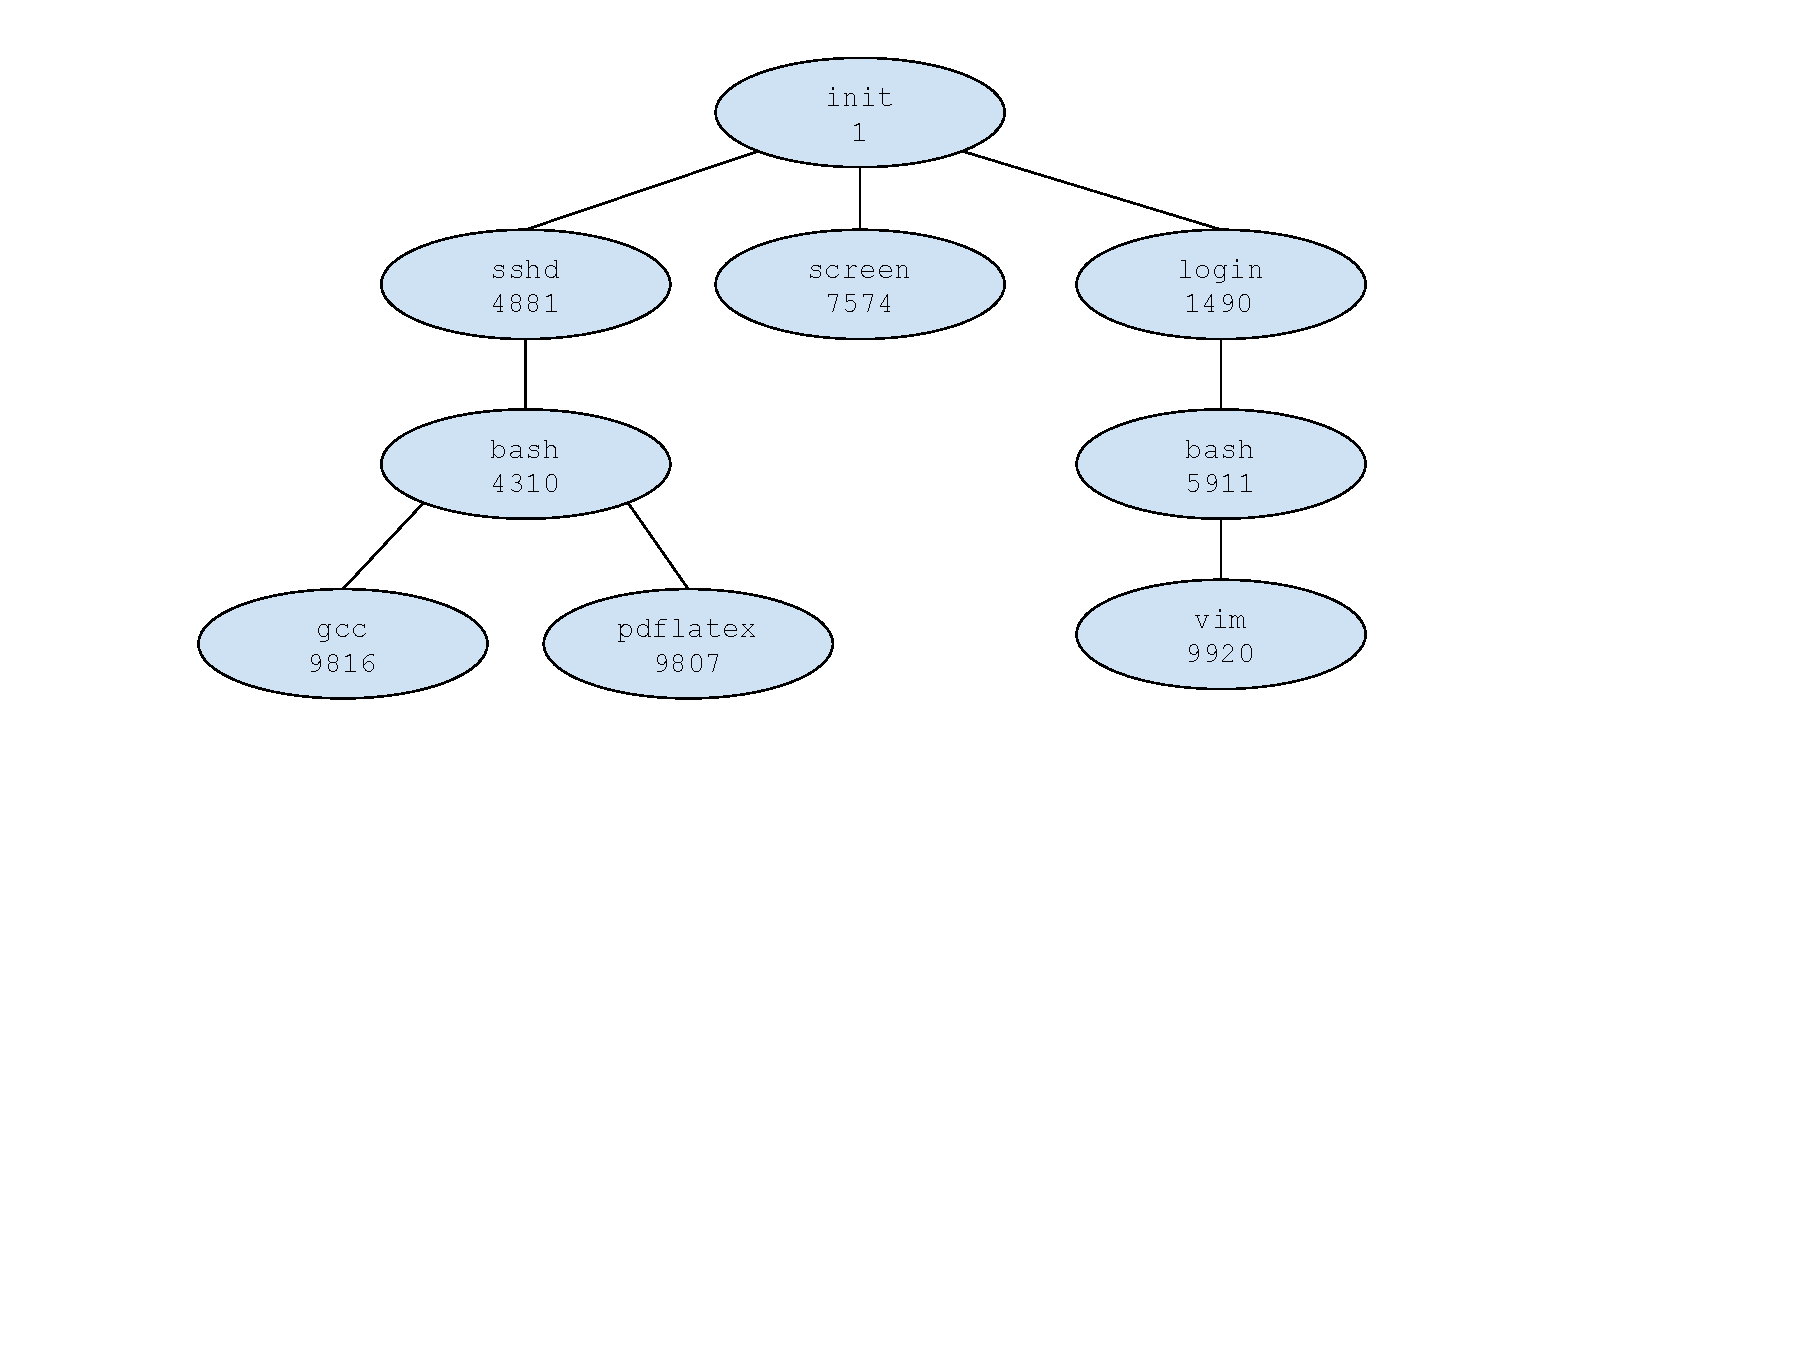
\includegraphics[width=\textwidth]{images/linux-process-tree.pdf}
\end{center}

\end{frame}

\begin{frame}
\frametitle{The \texttt{ps} Command}

We can obtain a list of processes with \texttt{ps}.

The diagram shows each user gets a \texttt{login} process.

The shell (\texttt{bash}) is spawned from \texttt{login}.

\end{frame}

\begin{frame}
\frametitle{Terminal Commands}

When you issue a command, like \texttt{ls} or \texttt{top} (table of processes), the new process is created and the shell will \texttt{wait} on that process.

It might finish on its own (e.g., \texttt{ls}).\\
\quad Or wait for the user to tell it to exit (\texttt{top})

When it does, control goes back to the shell.\\
\quad You get presented with the prompt again (e.g., \texttt{jz@Loki:\~{}/\$}).

Must I log in to the system in a second terminal window to run two things at a time? 

The answer is no, and there are two ways to get around it.

\end{frame}

\begin{frame}
\frametitle{Run in the Background}

Option 1: tell the shell we want the task to run in the background. 

To do that, add to the command the \texttt{\&} symbol: 

\texttt{gcc fork.c \&}

Control returns almost immediately to the shell.\\
\quad It is not waiting for \texttt{gcc} to finish.

\end{frame}

\begin{frame}
\frametitle{Run in the Background}

 You may see some output like \texttt{[1] 34429}.
 
This is the shell saying: child has been created; it has process ID 34429. 

When the process is finished, there is another update:

\texttt{[1]+  Done                    gcc fork.c}

\end{frame}

\begin{frame}
\frametitle{Run in the Background}

Notably, any console output that the \texttt{gcc} command would generate will still appear on the console where the background task was created. 

Maybe you want that but maybe you want to put the output in a log file, with a command like \texttt{cat fork.c > logfile.txt \&}. 

(Telling \texttt{gcc} to be silent is a somewhat more complex operation.) 

\end{frame}

\begin{frame}
\frametitle{The Cruel Ampersand}

The semantics of \texttt{\&} are not just ``run this in the background, please''.

It is actually the parent process (the shell) disowning its child. 

That process will get adopted by \texttt{init}.

It can run to completion even if the user logs out.


\end{frame}

\begin{frame}
\frametitle{Example of the \&}

A common example of a command I use involving the \texttt{\&}:\\
\texttt{ sudo service xyz start \& }

This will (with super user permissions) start up the service \texttt{xyz}.
	
It returns control to the console so I don't have to wait.

Next: \texttt{tail -f /var/log/xyz/console.log}

Watch the console log of the \texttt{xyz} service as it starts up.

\end{frame}

\begin{frame}
\frametitle{Option Two: \texttt{screen}}

The other alternative is the \texttt{screen} command. 

While having something run in the background is nice, it does not work for interactive processes. 

Example: text editing with \texttt{vi} and want to read e-mail with \texttt{pine}.

Could be done by saving and closing \texttt{vi}.

Or, start them in \texttt{screen} and switch between them.

\end{frame}

\begin{frame}
\frametitle{Using \texttt{screen}}
Instead of just opening \texttt{vi fork.c} I can issue the command \texttt{screen vi fork.c} and this spawns \texttt{screen} and takes me right to editing the file. 

The key difference is that I can ``detach'' from this screen and go back to the command line.

If I log out, \texttt{screen} keeps running with the \texttt{vi} inside it.

 If I have multiple screens running, I can just ``reattach'' to the one I want.

\end{frame}

\begin{frame}
\frametitle{Spawning Child Processes}

In general, when a process spawns a child, the child will need resources. 

The child may request them from the OS directly.

Or the parent can give some of its resources to the child. 

The parent may partition resources amongst the children or allow its children to share.

Restrict a child process to only some subset of its parent's resources?

 If so, cannot overload the system by spawning too many children.

\end{frame}

\begin{frame}
\frametitle{Spawning Child Processes}

At the time of initialization, the parent may pass the child some data.

Example: link from e-mail to browser.

Interesting note: child may be a duplicate or totally new.

\end{frame}

\begin{frame}
\frametitle{UNIX Workflow}

Parent spawns the child process with the \texttt{fork} system call. 

If waiting for the child process to finish, \texttt{wait}.\\
\quad Alternatively, carry on.

When the child process is finished, it returns a value with \texttt{exit} 

The parent gets this as the return value of \texttt{wait} and may proceed.
\end{frame}

\begin{frame}
\frametitle{About \texttt{fork}}

Note: \texttt{fork} creates a new process as a copy of itself.

Both parent and child continue after that statement.

The call \texttt{fork} can return a value:\\
\quad A negative value means the fork failed.\\
\quad A zero value means this process is the child.\\
\quad A positive value: this is the parent; the value is the child \texttt{pid}.

\end{frame}

\begin{frame}
\frametitle{After the \texttt{fork}, the \texttt{exec}}


After the \texttt{fork}, one of the processes may use the \texttt{exec} system call.

This will replace its memory space with a new program. 

There's no rule that says this must happen\\
\quad a child can continue to be a clone of its parent if it wishes.

The \texttt{exec} invocation loads a binary file into memory \& starts execution. 

At this point, the programs can go their separate ways.

Or the parent might want to wait for the child to finish.


\end{frame}

\begin{frame}[fragile]
\frametitle{Putting it Together}

{\scriptsize
\begin{verbatim}
int main()
{
  pid_t pid;
  int childStatus;

  /* fork a child process */
  pid = fork();
  
  if (pid < 0) { 
  
    /* error occurred */ 
    fprintf(stderr, "Fork Failed"); 
    return 1;
    
 } else if (pid == 0) { 
    /* child process */
    execlp("/bin/ls","ls",NULL);
    
  } else { 
    /* parent process */
    /* parent will wait for the child to complete */
    wait(&childStatus);
    printf("Child Complete with status: %i \n", childStatus);
    
  }
  return 0;
}
\end{verbatim}
}

\end{frame}

\begin{frame}[fragile]
\frametitle{Code Output}

Thus, the output is:
\begin{verbatim}
jz@Freyja:~/fork$ ./fork 
fork   fork.c
Child Complete with status: 0
jz@Freyja:~/fork$ 
\end{verbatim}


\end{frame}

\begin{frame}
\frametitle{Fork Visually}

Or, to represent this visually:

\begin{center}
\includegraphics[width=\textwidth]{images/fork-syscall.png}
\end{center}

\end{frame}

\begin{frame}
\frametitle{Termination?}

What about termination? 

On the assumption that the process is terminating normally and not being killed, the system call for that is \texttt{exit}. 

If the program itself has no explicit call to \texttt{exit}, the \texttt{return} statement at the end of \texttt{main} will have the same effect.

Let us modify that code above to fork off a child process that will exit ``abnormally'' with an exit code of 1. 

The \texttt{wait} function also returns the process ID of the child.

 This is so that the parent can identify which of its children has terminated, though it is not used in this example.

\end{frame}

\begin{frame}[fragile]
\frametitle{Abnormal Return Code}
{\scriptsize
\begin{verbatim}
int main()
{
  pid_t pid;
  int childStatus;

  /* fork a child process */
  pid = fork();
  
  if (pid < 0) { 
  
    /* error occurred */ 
    fprintf(stderr, "Fork Failed"); 
    return 1;
    
 } else if (pid == 0) {  
    /* child process */
    exit( 1 );
    
  } else {
    /* parent process */
    /* parent will wait for the child to complete */
    wait(&childStatus);
    printf("Child Complete with status: %i \n", childStatus);
    
  }   
  return 0;
}
\end{verbatim}

}

\end{frame}

\begin{frame}
\frametitle{UNIX System V Process Management}

UNIX divides its processes into two categories: system processes that run in kernel mode and user processes that run in user mode.

There are nine different states:

\begin{enumerate}
	\item \textbf{User Running}
	\item \textbf{Kernel Running}
	\item \textbf{Ready to Run, in Memory}
	\item \textbf{Asleep in Memory}
	\item \textbf{Ready to Run, Swapped}
	\item \textbf{Sleeping, Swapped}
	\item \textbf{Preempted}
	\item \textbf{Created}
	\item \textbf{Zombie}
\end{enumerate}


\end{frame}

\begin{frame}
\frametitle{UNIX Process States}

\begin{center}
\includegraphics[width=0.95\textwidth]{images/unix-states.png}
\end{center}

\end{frame}

\begin{frame}
\frametitle{UNIX Process Creation}

Process creation when \texttt{fork} is called means the OS does the following:

\begin{enumerate}
	\item It allocates a slot in the process table for the new process.
	\item It assigns a unique process ID to the child process.
	\item It makes a copy of the process image of the parent, with the exception of any shared memory.
	\item It increments counters for any files owned by the parent (showing there is an additional process referencing those files).
	\item The new process is in the state Ready to Run.
	\item A return value of 0 goes to the child process, and the unique process ID of the child is returned to the parent.
\end{enumerate}

\end{frame}

\begin{frame}
\frametitle{After the \texttt{fork}}

Afterwards, the system will need to choose which process is going to run: 

\begin{enumerate}
	\item The parent process. The child is in the ready to run state.
	\item The child process. The parent is in the ready to run state.
	\item Another process. Both parent and child are in the ready to run state.
\end{enumerate}

\end{frame}


\begin{frame}
\frametitle{Apr\`{e}s \texttt{fork}, le d\'{e}luge}

A short digression on a denial of service attack: the ``fork bomb''.

The idea is to call \texttt{fork} repeatedly.

Keep doing this until the system crashes (or no work can get done).

Exponential growth ($2^n$) processes after $n$ calls.

\end{frame}


\begin{frame}
\frametitle{Apr\`{e}s \texttt{fork}, le d\'{e}luge}
A system can be configured to defend against this.

1. Limit total number of processes per user.

2. Limit rate of process spawning.

Note: do not attempt this on University computers!

\end{frame}


\end{document}

